\documentclass[14pt]{article}

\usepackage[a4paper, left=2cm, right=2cm]{geometry} % A4 paper size and thin margins
% assinatura

\usepackage[signature=default_signature, nojob]{mysignature}

%--------
\usepackage{xcolor} % Required for specifying custom colours
\definecolor{grey}{rgb}{0.8,0.8,1} % Colour of the box surrounding the title

\usepackage[T1]{fontenc}
\usepackage[utf8]{inputenc} % Output font encoding for international characters
\usepackage[portuguese]{babel}
\usepackage{graphicx}
\usepackage[sfdefault]{ClearSans} % Use the Clear Sans font (sans serif)
%\usepackage{XCharter} % Use the XCharter font (serif)
\usepackage{fancyhdr}
\usepackage{dirtytalk}
\usepackage{listings}
\usepackage{xcolor}
\usepackage{float}
\usepackage{hyperref}
\hypersetup{
    colorlinks=true,
    linkcolor=cyan,
    filecolor=magenta,
    urlcolor=cyan,
}
\definecolor{blue}{rgb}{0.15,0.0,1.20}
\definecolor{codegreen}{rgb}{0,0.6,0}
\definecolor{codegray}{rgb}{0.5,0.5,0.5}
\definecolor{codepurple}{rgb}{0.58,0,0.82}
\definecolor{backcolour}{rgb}{0.95,0.95,0.91}

\lstdefinestyle{mystyle}{
    backgroundcolor=\color{backcolour},
    commentstyle=\color{codegreen},
    keywordstyle=\color{magenta},
    numberstyle=\tiny\color{codegray},
    stringstyle=\color{codepurple},
    basicstyle=\ttfamily\footnotesize,
    breakatwhitespace=false,
    breaklines=true,
    captionpos=b,
    keepspaces=true,
    numbers=left,
    numbersep=5pt,
    showspaces=false,
    showstringspaces=false,
    showtabs=false,
    tabsize=2
}

\lstset{style=mystyle}

\fancyhf{}
\pagestyle{fancy}
\rfoot{\thepage\hspace{1pt}}
\begin{document}

\begin{titlepage}

	\colorbox{grey}{
		\parbox[t]{0.93\textwidth}{ % Outer full width box
			\parbox[t]{0.91\textwidth}{ % Inner box for inner right text margin
				\raggedleft
				\fontsize{60pt}{70pt}\selectfont
				\vspace{0.5cm}

				FCT: Relatório do Curso de Prática Simulada\\


				\vspace{0.5cm}
			}
		}
	}
	\vfill

	\parbox[t]{0.93\textwidth}{
		\raggedleft
		\large
		{\Large
   	Escola Secundária António Damásio\\[4pt]
    \large Curso 2: Técnicas básicas de escrita de páginas dinâmicas em PHP\\[2pt]
    \large Tecnico de Gestão e Programação de Redes Informáticas: 2º Ano\\[2pt]
    \Large Diogo Valério}\\[4pt]
    Julho de 2020\\[1pt]
		\hfill\rule{0.6\linewidth}{1pt}
	}
\end{titlepage}


\tableofcontents
\newpage

\section{Introdução} \label{introducao}
Este relatório foi realizado no âmbito do curso de prática simulada facultado pela \textbf{ANPRI} (Associação Nacional Professores de Informática), a que fomos submetidos no lugar da
Formação em Contexto de Trabalho devido à pandemia de Covid-19 à qual estamos a passar de momento.

O curso frequentado foi o \textbf{Curso 2: Técnicas básicas de escrita de páginas dinâmicas em PHP} e decorreu de 19 de maio a
8 de julho, mas, devido a problemas técnicos na plataforma e também a ataques de \textit{Denial of Service}(também conhecido como \textit{DDOS})
à plataforma, o decorrer normal do curso foi prejudicado, sendo que este acabou por ser movido para a plataorma \textit{Google Sites}.


\section{Caracterização do Curso}
\subsection{Objetivos do Curso}
O curso teve como objetivo ensinar os alunos a
desenvolver páginas web dinâmicas com recurso à linguagem de programação PHP.
O curso também desenvolveu uma vertente de HTML para o desenvolvimento de páginas web e de SQL para a criação de bases de dados.

\subsection{Área de Atividade}
O curso foi hospedado primeiramente no \textit{moodle} da \textbf{ANPRI} e seguidamente na plataforma \textit{Google Sites}.

link para o curso no \textit{moodle} : \url{https://anpri.edu.pt/course/view.php?id=58}

link para o curso no \textit{Google Sites} : \url{https://sites.google.com/anpri.pt/cursodepraticasimuladaphp/}

\subsection{Contactos}
O curso foi dirigido pelo formador \textbf{Prof. Carlos Almeida} (prof.carlos.almeida@gmail.com) e foi o desenvolvido com a ajuda da \textbf{Prof. Ester Tavares} (ester.tro@gmail.com)

\section{Recursos Materiais}
Durante o decorrer do curso foram utilizados os seguintes materiais:

\subsection{Hardware}
\begin{list}{•}
\item Computador pessoal
\end{list}

\subsection{Software}

\subsubsection{Curso}
\begin{list}{•}
\item Editor: \textit{Atom};
\item
\item Servidor: \textit{Xampp};
\item SQL: \textit{phpMyAdmin}
\item Pasta Partilhada: \textit{GitHub}.
\end{list}

\subsubsection{Manual de Utilizador}
\begin{list}{•}
  \item Editor: \textit{Atom};
  \item
  \item Linguagem: \textit{Markdown};
  \item Edição de Imagem: \textit{Gimp}.
\end{list}


\subsubsection{Relatório}
\begin{list}{•}
\item Editor: \textit{Atom};
\item
\item Linguagem: \textit{LaTeX}.
\item Edição de Imagem: \textit{Gimp}.
\end{list}

\section{Descrição das Atividades Realizadas}
\subsection{1ª Semana}
Para a realização das fichas propostas na 1ª semana foi utilizado este manual de PHP fornecido pelo formador:

(\url{https://drive.google.com/file/d/1pBc5DzuNDO3r-SwA6CAJLiIEQJIsKn2r/view})

Durante a primeira semana foram desenvolvidos programas simples pois estes tinham como propósito ajudar-nos a perceber a sintaxe da linguagem PHP.
Entre estes programas estão:
\subsubsection{Programa que devolve uma mensagem}
Este programa teve como objetivo ensinar-nos a usar a função "\textbf{echo}".
\begin{lstlisting}[language=PHP]
  <!DOCTYPE html>
  <html lang="en" dir="ltr">
    <head>
      <meta charset="utf-8">
      <title></title>
    </head>
    <body>
      <?php echo "O primeiro programa nunca se esquece!"; ?>

    </body>
  </html>

\end{lstlisting}

\subsubsection{Programa que Devolve o Resultado de uma Operação Matemática}

Este programa teve como objetivo ensinar-nos a utilizar as Operações Matemáticas, neste caso, a Adição.

\begin{lstlisting}[language=PHP]
  <!DOCTYPE html>
  <html lang="en" dir="ltr">
    <head>
      <meta charset="utf-8">
      <title></title>
    </head>
    <body>
      <?php
  $a = 23;
  $b = 45;
  echo $a+$b;
  ?>

    </body>
  </html>


\end{lstlisting}

\subsubsection{Programa que Devolve a Tabuada de um Número}

Este programa teve como objetivo ensinar-nos a utilizar as estruturas de repetição, neste caso, o ciclo "\textbf{\textit{for}}".

\begin{lstlisting}[language=PHP]
  <!DOCTYPE html>
  <html lang="en" dir="ltr">
    <head>
      <meta charset="utf-8">
      <title></title>
    </head>
    <body>
  <?php
  $a = 4;
  for ($i=0; $i <= 12; $i++) {
    echo $a, "x",$i , "=" ,$a*$i, '<br \>';
  }
  ?>

    </body>
  </html>


\end{lstlisting}

\subsubsection{Programa que Devolve o Valor Presente num Espaço de um Array}

Este programa teve como objetivo ensinar-nos a utilizar arrays.

\begin{lstlisting}[language=PHP]
  <!DOCTYPE html>
  <html lang="en" dir="ltr">
    <head>
      <meta charset="utf-8">
      <title></title>
    </head>
    <body>
  <?php

  $cores = array('Vermelho', 'Verde', 'Azul', 'Violeta');
  echo $cores[1];

  ?>

    </body>
  </html>

\end{lstlisting}

\subsubsection{Programa que Cria um formulário}

Este programa teve como objetivo ensinar-nos a utilizar formulários em conjunto com os métodos \textbf{POST} e \textbf{GET}.

\begin{lstlisting}[language=PHP]
  <!DOCTYPE html>
  <html lang="en" dir="ltr">
    <head>
      <link rel="stylesheet" href="style.css">
      <meta charset="utf-8">
      <title></title>
    </head>
    <body>
      <?php ?>
      <fieldset>
        <form action="tratamento.php" method="post">
          <table>
          <tr>
        <label for="nome">Nome: </label> <input type = "text" name="nome"><br>
        <label for="email">Email: </label> <input type = "email" name = "email"><br>
        <label for="telefone">Telefone/Telemóvel: </label> <input type = "text" name = "telefone"><br>
        <br>
        <br>
            <td align = "left">
              Cursos de informatica:
            </td align = "left">
            <td>
               <input name = "cursos" type="radio"  value="Android" > Android
               <br>
               <input name = "cursos"type="radio" value="Html" > Html
               <br>
               <input name = "cursos" type="radio"  value="Java"> Java
               <br>
               <input name = "cursos" type="radio"  value="PHP" > PHP
               <br>
               <input name = "cursos" type="radio" value="Python"> Python
               <br>
               <input name = "cursos" type="radio" value="SQL" > SQL
               <br>
               <input name = "cursos" type="radio" value="Scratch" > Scratch
               <br>
               <br>
             </td>
             <tr>
                <td>
                  <label for="nivel">Selecione uma opção:</label>
                </td>
                <td align="left">
                    <select name="nivel">
                      <option value="init">Iniciação</option>
                      <option value="med">Intermédio</option>
                      <option value="adv">Avançado</option>
                    </select>
                </td>
             </tr>

             <tr>
                <td>
                  <br>
                  <br>
                  <br>
                  <label for="obs">Observações:</label>
                  <textarea name="obs"></textarea>
                </td>
            </tr>

          </tr>
        </table>
        <input type="submit" name="submit" value="Enviar">
        </form>
      </fieldset>
    </body>
  </html>
\end{lstlisting}

\subsubsection{Programa que Define COOKIES e em Seguida Devolve-as}

Este programa teve como objetivo ensinar-nos a utilizar \textbf{COOKIES}.

\begin{lstlisting}[language=PHP]
  <!DOCTYPE html>
  <html lang="en" dir="ltr">
    <head>
      <meta charset="utf-8">
      <title></title>
    </head>
    <body>
      <?php

      $cookies['nome'] = 'joao';
      $cookies['Apelido'] = 'Alberto';
      $cookies['idade'] = '20';
      $cookies['morada'] = 'rua das 12 casas nr 13';

      foreach($cookies as $key => $value) {
        setcookie($key,$value, time()+3600);
      }
      echo "<hr /><pre>";print_r($_COOKIE);echo '<pre>';
      ?>
    </body>
  </html>

\end{lstlisting}

\subsubsection{Programa que Define Variávies de Sessão por Meio de um Formulário e em Seguida Devolve-as}

Este programa teve como objetivo ensinar-nos a utilizar \textbf{Sessões}.

\begin{lstlisting}[language=PHP]
  <!DOCTYPE html>
  <html lang="en" dir="ltr">
   <head>
     <meta charset="utf-8">
     <title></title>
   </head>
   <body>
     <form name = "form" action="" method="post">
       Nome:
       <input type = "text" name = "name">
       <input type = "submit" value= "Iniciar Sessão" name="sendform">
     </form>
     <?php
       if(isset($_SESSION['sendform'])){
         $ses['id'] = session_id();
         $ses['on'] = time();
         $ses['off'] = time() + 30;
         $ses['ip'] = $_SERVER['REMOTE_ADDR'];
         $ses['nome'] = $_POST['nome'];

         $_SESSION['user'] = $ses;

         header('Location'.$_SERVER['PHP_SELF']);
       }

       if(empty($_SESSION['user'])){
         echo '<form name = "form" action="" method="post">
               Nome:
               <input type = "text" name = "name">
               <input type = "submit" value= "Iniciar Sessão" name="sendform">
               </form>';
       }
       else{
         $tempoLog = $_SESSION['user']['on'];
         $tempoAgora = time();
         $tempoOnLine = $tempoAgora - $tempoLog;
         $tempoFim = $_SESSION['user']['off'] - $tempoAgora;
         echo 'ola'.$_SESSION['user']['nome'].' Esta logado a '.$tempoLog.'segundos';
         echo 'O seu IP é'.$_SESSION['user']['ip'];
       }
     ?>
   </body>
  </html>
\end{lstlisting}

\subsection{2ª Semana}

Para a realização das fichas propostas na 2ª semana foi utilizado este manual de PHP fornecido pelo formador:

(\url{https://drive.google.com/file/d/1KPxefR_ecFTfHb6bireXgTzu93E6CVRZ/view})

Durante a 2ª semana houve a abordagem da linguagem SQL de maneira a ensinar os alunos a criar e manipular bases de dados relacionais.
Alguns exemplos da sua utilização são:

\subsubsection{Criação de Tabelas Relacionadas }

\begin{lstlisting}[language=SQL]
  create table Colaborador(
    nomeColaborador char(30) PRIMARY KEY,
    morada char(30) not null,
    cidade char(15) not null,
    estadoCivil char(15) not null );

  create table Empresa(
    nomeEmpresa char(30) PRIMARY KEY,
    cidade char(15) not null );

    create table Trabalha(
    	nomeColaborador char(30),
    	nomeEmpresa char(30),
    	salario float not null ,
    	FOREIGN key(nomeColaborador) REFERENCES Colaborador(nomeColaborador),
      FOREIGN key(nomeEmpresa) REFERENCES Empresa(nomeEmpresa),
      PRIMARY KEY(nomeColaborador,nomeEmpresa)
    );

    create table Diretor(
      	nomeColaborador char(30),
      	nomeEmpresa char(30),
      	FOREIGN key(nomeColaborador) REFERENCES Colaborador(nomeColaborador),
        FOREIGN key(nomeEmpresa) REFERENCES Empresa(nomeEmpresa),
        PRIMARY KEY(nomeColaborador,nomeEmpresa)
    );

\end{lstlisting}
\newpage
\subsubsection{Criação de Utilizadores e Definição dos seus Privilégios}

\begin{lstlisting}[language=SQL]
  CREATE USER CAntunes IDENTIFIED BY 'CAntunes?218';
  CREATE USER ASilva IDENTIFIED BY 'ASilvs!109';
  GRANT All PRIVILEGES  ON Colaborador.* TO CAntunes;
  GRANT SELECT ON Colaborador.* TO ASilva;
\end{lstlisting}

\subsubsection{Criação de Uma Base de Dados Relacional }

\begin{lstlisting}[language=SQL]
create database Pais;


create table Distrito(
  CodDistrito int Auto_increment PRIMARY KEY,
  nomeDistrito varchar(30),
  AreaTotal float not null,
  População int not null
);

create table Provincia(
  CodProvincia int Auto_increment PRIMARY KEY,
  nomeProvincia varchar(30) not null,
  DescricaoPorvincia varchar(250)not null
);

create table Concelho(
  CodConcelho int Auto_increment PRIMARY KEY,
  CodDistrito int not null,
  nomeConcelho varchar(30) not null,
  CodProvincia int not null,
  FOREIGN key(CodDistrito) REFERENCES Distrito(CodDistrito),
  FOREIGN key(CodProvincia) REFERENCES Provincia(CodProvincia)
);

insert into Distrito(nomeDistrito, AreaTotal, Populacao) values('Lisboa', 2761, 3079772);
insert into Distrito(nomeDistrito, AreaTotal, Populacao) values('Leiria', 3506, 470895);
insert into Distrito(nomeDistrito, AreaTotal, Populacao) values('Aveiro', 2798.54, 714200);
insert into Distrito(nomeDistrito, AreaTotal, Populacao) values('Castelo Branco', 6675, 196264);
insert into Distrito(nomeDistrito, AreaTotal, Populacao) values('Coimbra', 3947, 429987);

insert into Provincia(nomeProvincia, DescricaoPorvincia)
values('Estremadura', 'A Estremadura é uma província histórica (ou região natural) de Portugal, estabelecida na Idade Média e extinta no século XIX, devendo o seu nome derivar do latim Extrema Durii');
insert into Provincia(nomeProvincia, DescricaoPorvincia)
values('Beira Litoral', 'A Beira Litoral é uma província histórica (ou região natural) situada na região do Centro de Portugal, formalmente instituída por uma reforma administrativa havida em 1936.');
insert into Provincia(nomeProvincia, DescricaoPorvincia)
values('Beira Baixa', 'A Beira Baixa é uma província histórica (ou região natural) situada na região do Centro de Portugal, originalmente criada no século XIX a partir de parte do território da anterior Província da Beira.');
insert into Provincia(nomeProvincia, DescricaoPorvincia)
values('Beira Alta', 'A Beira Alta é uma província histórica (ou região natural) situada na região do Centro de Portugal. Foi criada, em 1832, por subdivisão da antiga província da Beira, passando a ser constituída pelas comarcas de Viseu, Lamego e Trancoso.');
insert into Provincia(nomeProvincia, DescricaoPorvincia)
values('Douro Litoral', 'O Douro Litoral é uma província histórica de Portugal, formalmente instituída por uma reforma administrativa havida em 1936.');

insert into Concelho(CodDistrito, nomeConcelho, CodProvincia) values(1,'Alcobaça',1);
insert into Concelho(CodDistrito, nomeConcelho, CodProvincia) values(2,'Alcobaça',1);
insert into Concelho(CodDistrito, nomeConcelho, CodProvincia) values(3,'Castelo de Paiva',2);
insert into Concelho(CodDistrito, nomeConcelho, CodProvincia) values(4,'Fundão',3);
insert into Concelho(CodDistrito, nomeConcelho, CodProvincia) values(5,'Arganil',3);

\end{lstlisting}


\subsection{3ª Semana}
Para a realização das fichas propostas na 3ª semana foi utilizado o mesmo manual de PHP da 1ª semana:

(\url{https://drive.google.com/file/d/1KPxefR_ecFTfHb6bireXgTzu93E6CVRZ/view})

Durante a 3ª semana foi trabalhada a ligação a sockets criando clientes e servidores.
Um exemplo dos exercicios desenvolvidos é:

\subsubsection{Servidor e Cliente que }

\begin{lstlisting}[language=PHP]
  <?php
    error_reporting(E_ALL);
    set_time_limit(0);
    ob_implicit_flush();
    $address = "127.0.0.1";
    $port = "8887";
    $cliente = array();
    if( ($sock = socket_create(AF_INET, SOCK_STREAM, 0)) === false){
      echo "ERRO - Falha na criação do socket! \n".
      socket_strerror(socket_last_error())."\n";
    }
    if(socket_bind($sock, $address, $port) === false){
      echo "ERRO - Falha na passagem do Endereço e porta para o socket! \n".
      socket_strerror(socket_last_error($sock))."\n";
    }
    if(socket_listen($sock) === false){
      echo "ERRO - Falha na escuda da ligação ao socket! \n".
      socket_strerror(socket_last_error($sock))."\n";
    }
  do{
    echo "\nA esperar por clientes...\n";
    $read = array();
    $read[] = $sock;
    $write = array();
    $expect = array();
    $tv_sec = NULL;
  	$cont = 0;
  	$maxClientes = 2;
    $read = array_merge($read, $cliente);
    if(socket_select($read, $write, $expect, $tv_sec) === false){
      echo "ERRO - Falha ao aceitar a ligação ao socket! ".
      socket_strerror(socket_last_error($sock))."\n";
      continue;
    }
    if(in_array($sock, $read)){
      if(($msgsock = socket_accept($sock)) === false){
        echo "ERRO - Falha ao aceitar a ligação ao socket! ".
        socket_strerror(socket_last_error($sock))."\n";
        break;
      }
      $cliente[] = $msgsock;
      $key = array_keys($cliente, $msgsock);
  		$cont = count($cliente);
  		if ($cont > $maxClientes) {
  			echo "Nova ligacao recusada. O servidor chegou ao maximo de ", $maxClientes, " ligacoes";
  			$msgmax = "O servidor não permite mais ligações";
  			socket_write($msgsock, $msgmax, strlen($msgmax));
  			socket_close($client);
  			unset($cliente[$key]);
  		}
  		socket_getpeername($msgsock, $ip);
      echo "\n Um cliente com ip ",$ip," estabeleceu a ligação - cliente numero: $key[0]\n";
  		echo "Neste momento esta(ao) " ,$cont, " clientes conectado(s) ao servidor";
      $msg = "\n Bem-Vindo ao PHP server socket V2 - Multi - Cliente. \n\r".
      "Voce é o cliente numero: $key[0] \n\r".
      "Para sair, digite 'quit'. Para desligar o servidor digite 'shutdown'. \n\r";
      socket_write($msgsock, $msg, strlen($msg));
    }
    foreach ($cliente as $key => $client) {
      if(in_array($client, $read)){
        if(($buf = socket_read($client, 2048, PHP_NORMAL_READ)) === false){
          echo "ERRO- Falha na leitura do socket! ".
          socket_strerror(socket_last_error($client))."\n";
          break 2;
        }
        if(!$buf = trim($buf)){
          continue;
        }
        if($buf == 'quit'){
  				echo "\n O cliente $key disconectou-se!\n";
  				socket_close($client);
          unset($cliente[$key]);
          break;
        } else if($buf == 'shutdown'){
            socket_shutdown($sock);
          }
        $talkback = "Cliente $key disse: '$buf' \n";
  			foreach ($cliente as $key2) {
  				socket_write($key2,$talkback, strlen($talkback));
  			}
        echo "Cliente $key disse: '$buf' \n";
      }
    }
  }while(true);
  socket_close($sock);
  echo "o servidor encerrou";
?>
\end{lstlisting}


\subsection{4ª Semana}

Para a realização do Projeto Final na 4ª semana foi utilizado este artigo do blog pessoal da Prof. Ester Tavares:

(\url{https://bdprogramacao.blogspot.com/2020/03/conexao-base-de-dados-no-phpmyadmin.html})

Durante a 4ª Semana foi desenvolvido o Projeto Final do curso.
Este consistia em desenvolver uma base de dados relacional em SQL e em seguida um site para fazer a sua manipulação.
A integração do site com a base de dados foi feita na linguagem PHP.

Para a criação deste Projeto Final foi utilizado \href{https://getbootstrap.com/}{\textbf{\textit{Bootstrap 4}}} para facilitar o design do site e a implementação do mesmo:


O código fonte do Projeto está disponível neste endereço:

(\url{https://github.com/Valerioooo/fichas/tree/master/ProjetoFinal/})


\newpage
\section{Reflexão Final}

No inicio do curso as atividades foram bem definidos como mostra a figura seguinte:

\begin{figure}[H]
    \centering
    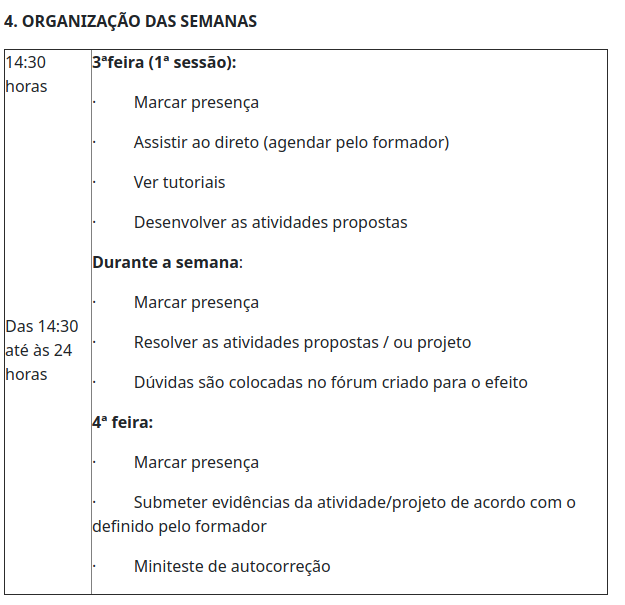
\includegraphics[width=0.45\linewidth]{cal.png}
    \caption{Calendário da primeira semana}
    \label{fig:cal}
\end{figure}


\subsection{Formador}

\begin{itemize}
  \item No primeiro dia (3ª feira) apenas existia forma de marcar presença para o segundo (4ª feira) e no dia seguinte foi adicionada a marcação de presença para o dia anterior;
  \item Não existiram atividades propostas nos primeiros dias;
  \item Não existiu qualquer interação entre o formador e os alunos durante as primeiras duas semanas;
  \item Apenas no final da 2ª semana teve lugar uma reunião na plataforma \textit{Zoom}, à qual nem eu nem muitos alunos fomos convidados/notificados. Esta acabou por não ser efetuada pois o limite da plataforma é de 100 participantes enquanto o numero de alunos do curso excedia os 200;
  \item O formador não respondeu a nenhuma dúvida no forum de dúvidas até ao final da 2ª semana do curso;
  \item Nunca existiu qualquer tipo de teste ou \say{miniteste} durante o decorrer do curso.
\end{itemize}
\newline
\subsection{Organização do curso}
\begin{itemize}
  \item As fichas fornecidas aos alunos não eram claras em certos aspetos, nomeadamente, o facto das fichas pedirem input do utilizador, não sendo clara a forma de o fazer e ainda, pedir a utilização de funções da linguagem PHP que não estavam descritas nos manuais fornecidos e com uma implementação pouco clara na própria documentação oficial da linguagem.
  \item Não existiu qualquer resposta da ANPRI em relação aos problemas enfrentados na utilização do site devido aos ataques sucessivos descritos no ponto \large\ref{introducao}.
\end{itemize}

Com decorrer do curso encontrei poucas dificuldades associadas às fichas, exceto na ficha em que eram tratados os \textit{Sockets}.
Como o servidor Xampp não habilita os \textit{Sockets} por defeito, é importante habilita-los:
\begin{itemize}
  \item Se o Sistema Operativo utilizado for \textit{Windows} pode ser efetuada por meio da edição do ficheiro php.ini, descomentando a linha \textit{\say{extension=php\_sockets.dll}}  no mesmo.
  \item Caso o Sistema Operativo utilizado for MacOS ou Linux é nessessária a compilação do código fonte da linguagem PHP com a \textit{flag} \textit{\say{--enable-sockets}}.
\end{itemize}


\subsection{Satisfação em Relação ao Curso}

O curso foi bastante interessante pois proporcionou-me uma aprendizagem autónoma com recurso à documentação específica das ferramentas, tutoriais em vídeo e a fóruns de programação na internet.

Na minha opinião a parte mais interessante do curso foi o Projeto Final, pois levou-me descobrir a ferramenta {\textbf{\textit{Bootstrap}} que se revelou uma grande ajuda ao desenvolvimento do Site.

Gostaria de agradecer à escola por me ter proporcionado este curso de modo a concluir este ano letivo. Agradeço especialmente à Prof. Ester Tavares que me apoiou em todo o processo de estágio, recomendando e orientando na escolha das ferramentas a utilizar e na execução das fichas.
\subsection{Avaliação}
Pelo facto de ter entregue todos os trabalhos completos no devido prazo e por ter consciência de que executei as tarefas com o maior zelo pela qualidade das mesmas, penso que mereço uma nota de fim de estágio não inferior a 18 valores.
\newline
\begin{figure}[H]
    \centering
    
\includegraphics[width=0.60\linewidth]{certificado.png}
    \caption{Certificado do Curso}
    \label{fig:certificado}
\end{figure}


\mysignature[left]{full}


\end{document}
